% Preview of the Experiment 2 thesis assets. Preamble: the packages of the thesis's
% dissertation.tex that tables and figures use (uathesis print layout: A4, 12 pt, scale 0.75,
% 5 mm binding offset). algorithm.sty is omitted (not installed on this machine; unused here).
\documentclass[a4paper,12pt,openany]{book}
\usepackage[a4paper,hmarginratio=1:1,vmarginratio=1:1,scale=0.75,bindingoffset=5mm]{geometry}
\usepackage{graphicx}
\usepackage{cmap}
\usepackage{amssymb}
\usepackage{amsmath}
\usepackage{setspace}
\usepackage{booktabs}
\usepackage{url}
\usepackage{adjustbox}
\usepackage{tabularx}
\usepackage{tabularray}
\usepackage{multicol}
\usepackage{subcaption}
\usepackage[inline]{enumitem}
\usepackage[table,usenames,dvipsnames]{xcolor}
\usepackage{rotating}
\usepackage{makecell}
\usepackage[unicode=true,colorlinks=true,linkcolor=black]{hyperref}
\usepackage{cleveref}
\newcolumntype{Y}{>{\centering\arraybackslash}X}
\renewcommand\floatpagefraction{.9}
\renewcommand\topfraction{.9}
\renewcommand\bottomfraction{.9}
\renewcommand\textfraction{.1}
\setcounter{totalnumber}{50}
\setcounter{topnumber}{50}
\setcounter{bottomnumber}{50}
\begin{document}
\chapter*{Experiment 2: tables and figures (preview)}
Generated by \texttt{experiments/exp2\_thesis/make\_assets.py}. References:
Tables~\ref{tab:exp2-headline}--\ref{tab:exp2-s8-families}, Figures~\ref{fig:exp2-auc}--\ref{fig:exp2-heart-pairs}.

\section*{Headline}
% Generated by experiments/exp2_thesis/make_assets.py -- do not edit by hand.
\begin{table}[tbp]
  \centering
  \small
  \begin{tabularx}{\textwidth}{@{}>{\raggedright\arraybackslash}Xccc@{}}
    \toprule
     & Adult & Churn & Heart-100 \\
    \midrule
    Registration & pre-registered & supplementary & supplementary \\
    Inputs & 107 & 71 & 26 \\
    Training / test rows & 39{,}073 / 9{,}769 & 4{,}000 / 1{,}000 & 242 / 61 \\
    Generations per seed & 100 & 100 & 100 \\
    \midrule
    Train AUC, median (range) & 0.909 (0.906--0.913) & 0.903 (0.892--0.919) & 0.956 (0.951--0.964) \\
    Test AUC, median (range) & 0.906 (0.903--0.909) & 0.886 (0.873--0.904) & 0.892 (0.863--0.926) \\
    Test AUC of LR / GB (same split) & 0.905 / 0.928 & 0.813 / 0.934 & 0.919 / 0.945 \\
    Seeds within 0.01 of the best seed & 10/10 & 4/10 & 1/10 \\
    \midrule
    Hidden units, median (range) & 15 (11--17) & 17 (13--27) & 8.5 (5--13) \\
    Explained to full coverage & 10/10 & 10/10 & 10/10 \\
    \quad within the 3-hour box & 10/10 & 10/10 & 10/10 \\
    Recheck complete (mismatches) & 10/10 (0) & 10/10 (0) & 10/10 (0) \\
    Agent explaining minutes, median (range) & 21.5 (19.3--28.8) & 18.1 (15.7--24.4) & 14.9 (12.5--16.5) \\
    Verified by Mike & 10/10 & 10/10 & 10/10 \\
    \quad minutes per network, median (range) & 4 (2--8)$^\ast$ & 3.5 (1--8) & 5.5 (3--10) \\
    \bottomrule
  \end{tabularx}
  \caption{Experiment~2: ten seeds per study, each seed's best network by training fitness. Test AUC is of that network on the held-out rows. LR is $L_2$ logistic regression and GB tuned gradient boosting, both fitted on the same split. A seed is within 0.01 of the best seed when its test AUC is at most 0.01 below the best seed's. Explanations used the frozen v4 method, one explaining agent per network; the recheck reran every stored query. $^\ast$Minutes recorded for 9 of the 10 Adult networks (not for s3).}
  \label{tab:exp2-headline}
\end{table}

% Generated by experiments/exp2_thesis/make_assets.py -- do not edit by hand.
\begin{figure}[tbp]
  \centering
  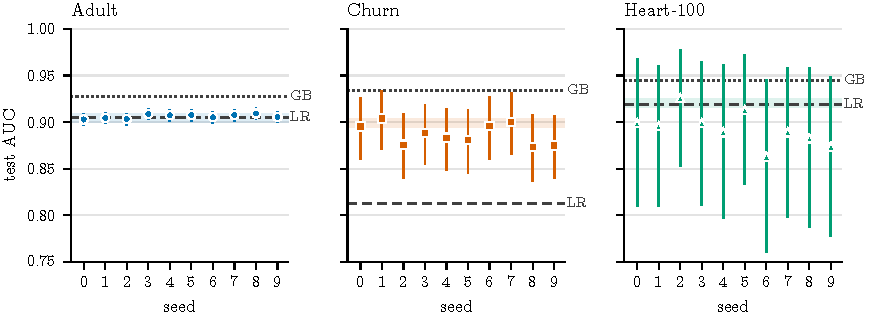
\includegraphics[width=\textwidth]{figures/exp2/exp2-auc}
  \caption{Test AUC of each seed's network, with its 95\% bootstrap interval. Shaded: within 0.01 of the best seed. Dashed: logistic regression (LR); dotted: tuned gradient boosting (GB), both on the same split. Seeds within 0.01 of the best: Adult 10/10, Churn 4/10, Heart-100 1/10. Test rows: Adult 9{,}769, Churn 1{,}000, Heart-100 61.}
  \label{fig:exp2-auc}
\end{figure}

% Generated by experiments/exp2_thesis/make_assets.py -- do not edit by hand.
\begin{figure}[tbp]
  \centering
  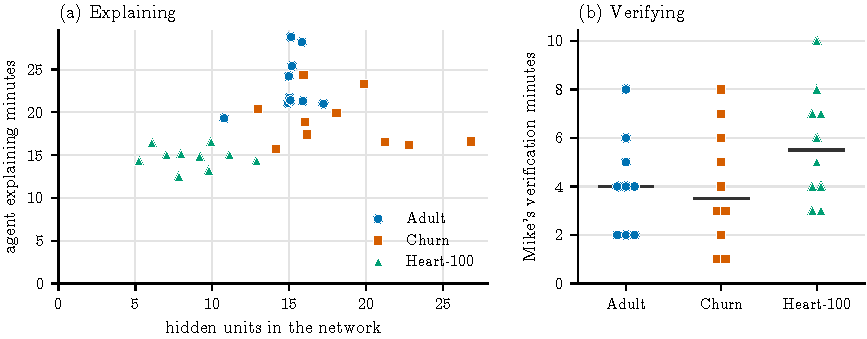
\includegraphics[width=\textwidth]{figures/exp2/exp2-cost}
  \caption{Cost of explaining and verifying, one mark per network. (a) The explaining agent's wall-clock minutes against network size (12.5 to 28.8 minutes). (b) Mike's minutes to verify each explanation (1 to 10; bar: median per study), using the plain-language report, the pairs plot and the expandable network; minutes were not recorded for Adult s3.}
  \label{fig:exp2-cost}
\end{figure}

\clearpage
\section*{Heart}
% Generated by experiments/exp2_thesis/make_assets.py -- do not edit by hand.
\begin{table}[tbp]
  \centering
  \footnotesize
  \begin{tabularx}{\textwidth}{@{}>{\raggedright\arraybackslash}X>{\raggedright\arraybackslash}p{3.3cm}ccc@{}}
    \toprule
    Model & Settings & Test AUC & 95\% interval & CV AUC \\
    \midrule
    \multicolumn{5}{@{}l}{\textit{PropNEAT networks}} \\
    The paper's Heart network (40 generations) & -- & 0.897 & [0.808, 0.966] & -- \\
    Heart-100, best seed (s2) & -- & 0.926 & [0.853, 0.978] & -- \\
    Heart-100, median of ten seeds & -- & 0.892 & range 0.863--0.926 & -- \\
    Heart-100, mean prediction of ten seeds & -- & 0.904 & -- & -- \\
    \midrule
    \multicolumn{5}{@{}l}{\textit{Comparators, tuned by 5-fold CV on the training rows}} \\
    Random forest & depth~5, min.\ leaf~5 & 0.949 & [0.887, 0.991] & 0.900 \\
    Explainable boosting machine & interactions~0, bins~32 & 0.947 & [0.886, 0.990] & 0.902 \\
    Gradient boosting, tuned & $L_2$~1, rate~0.03, iterations~100, leaves~7, min.\ leaf~20 & 0.945 & [0.885, 0.988] & 0.888 \\
    Logistic regression ($L_1$, sparse) & $C$~0.3 & 0.926 & [0.849, 0.983] & 0.905 \\
    Logistic regression ($L_2$) & $C$~0.1 & 0.919 & [0.841, 0.978] & 0.905 \\
    Gradient boosting, default settings & -- & 0.918 & -- & -- \\
    MLP, one hidden layer & $\alpha$~1, hidden units~8 & 0.904 & [0.819, 0.969] & 0.888 \\
    Decision tree & depth~6, min.\ leaf~10 & 0.855 & [0.750, 0.944] & 0.823 \\
    \bottomrule
  \end{tabularx}
  \caption{Heart on the paper's split (242 training and 61 test patients). Intervals are 95\% percentile intervals from 10{,}000 bootstrap resamples of the test set (seed 42). CV AUC is the cross-validated AUC on the training rows that chose the settings. The median of ten seeds is not one network, so its range across seeds is given instead of an interval. With 61 test patients the intervals are about 0.1 wide and overlap throughout.}
  \label{tab:exp2-heart-benchmark}
\end{table}

% Generated by experiments/exp2_thesis/make_assets.py -- do not edit by hand.
\begin{table}[tbp]
  \centering
  \small
  \textit{(a) Full against linearised networks}\par\smallskip
  \begin{tabular}{@{}lccc@{}}
    \toprule
    Mean over the ten networks & Full network & Linearised & Gain \\
    \midrule
    Train AUC (242 patients) & 0.956 & 0.927 & $+$0.029 \\
    Test AUC (61 patients) & 0.893 & 0.891 & $+$0.002 \\
    \bottomrule
  \end{tabular}
  \par\bigskip
  \textit{(b) Every non-linear unit and part}\par\smallskip
  \begin{adjustbox}{max width=\textwidth}
  \begin{tabular}{@{}lcccccc@{}}
    \toprule
    & Total & \makecell{Test gain\\CI $>0$} & \makecell{No measurable\\test effect} & Recurring & \makecell{Seed-\\specific} & \makecell{Small support\\($n<30$)} \\
    \midrule
    Non-linear units & 62 & 1 & 61 & 19 & 28 & 16 \\
    Non-linear parts & 45 & 1 & 44 & 9 & 27 & 6 \\
    \bottomrule
  \end{tabular}
  \end{adjustbox}
  \caption{Heart-100 audit: how much of the ten networks' non-linear structure shows on new patients. (a) Each network against itself with every non-linear unit replaced by its best straight line on the training rows; 93\% of the mean training gain does not carry over to the test set, the linearised network does as well or better on test in 5 of 10, and no network has a test-gain interval above zero. (b) A unit or part \emph{generalises} when its own test gain has a 95\% interval above zero; \emph{recurring} means another seed's network reproduces its non-linear residual. Units and parts too close to linear to match (15 and 9) are counted in neither. Binary one-step units are treated as linear. Exploratory, not pre-registered; test numbers were never used to choose.}
  \label{tab:exp2-heart-audit}
\end{table}

% Generated by experiments/exp2_thesis/make_assets.py -- do not edit by hand.
\begin{figure}[tbp]
  \centering
  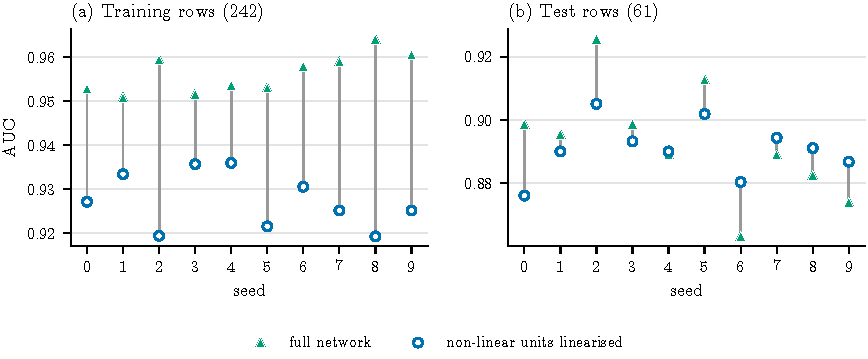
\includegraphics[width=\textwidth]{figures/exp2/exp2-heart-linearised}
  \caption{Heart-100: each network's AUC with and without its non-linear units (each replaced by its best straight line on the training rows). The non-linear units add 0.029 training AUC on average but 0.002 on test, and in 5 of the ten networks the linearised version does as well or better on test.}
  \label{fig:exp2-heart-linearised}
\end{figure}

% Generated by experiments/exp2_thesis/make_assets.py -- do not edit by hand.
\begin{table}[tbp]
  \centering
  \footnotesize
  \begin{tabularx}{\textwidth}{@{}>{\raggedright\arraybackslash}X>{\raggedright\arraybackslash}p{1.5cm}ccccc@{}}
    \toprule
    Family & Seeds & Units & \makecell{Raises /\\lowers risk} & \makecell{Train gain,\\median (max)} & \makecell{Test gain,\\range of estimates} & \makecell{Test CI\\$>0$ / $<0$} \\
    \midrule
    Thallium scan (with ST depression) & s0, s2, s5, s7, s8, s9 & 13 & 10 / 3 & $+$0.0046 ($+$0.0336) & $-$0.001 to $+$0.012 & 0 / 0 \\
    Thallium scan $\times$ age & s2 & 2 & 1 / 1 & $+$0.0057 ($+$0.0093) & $+$0.014 to $+$0.034 & 1 / 0 \\
    Resting blood pressure & s3, s4, s5, s8 & 7 & 4 / 3 & $+$0.0004 ($+$0.0082) & $-$0.005 to $+$0.004 & 0 / 0 \\
    Exercise angina & s0, s4, s6, s9 & 7 & 3 / 4 & $+$0.0072 ($+$0.0163) & $-$0.017 to $+$0.004 & 0 / 0 \\
    Age & s2, s3, s8, s9 & 6 & 1 / 5 & $+$0.0044 ($+$0.0095) & $-$0.006 to $+$0.012 & 0 / 0 \\
    \bottomrule
  \end{tabularx}
  \caption{Heart-100 audit: the non-linear units whose switch is driven by the four inputs of interest, by family. A unit belongs to the family of the inputs that flip it on or off; \emph{raises} or \emph{lowers} is the effect of the unit being on, relative to its straight-line fit. Gains are in AUC when the unit is linearised (train) and on the 61 test patients. The thallium gates recur in idea across seeds but not in mechanism, and none of these families has a measurable test effect, apart from one thallium $\times$ age unit (s2).}
  \label{tab:exp2-heart-families}
\end{table}

% Generated by experiments/exp2_thesis/make_assets.py -- do not edit by hand.
\begin{table}[tbp]
  \centering
  \footnotesize
  \begin{adjustbox}{max width=\textwidth}
  \begin{tabular}{@{}llcccccc@{}}
    \toprule
    & & \multicolumn{2}{c}{Linear path} & \multicolumn{3}{c}{Average effect, all ten networks} & \\
    \cmidrule(lr){3-4}\cmidrule(lr){5-7}
    Input & Per & \makecell{Networks\\($+$ / $-$)} & Same sign & $+$ / $-$ & Median (min to max) & Spread & LR \\
    \midrule
    Age & year & 9 (8 / 1) & mostly & 10 / 0 & $+$0.024 ($+$0.0019 to $+$0.06) & 31-fold & $+$0.014 \\
    Female (vs male) & level & 9 (0 / 9) & yes & 0 / 10 & $-$2.22 ($-$2.61 to $-$1.34) & 2-fold & $-$1.92 \\
    Typical angina & level & 10 (0 / 10) & yes & 0 / 10 & $-$2.46 ($-$3.76 to $-$0.95) & 4-fold & $-$2.10 \\
    Atypical angina & level & 10 (1 / 9) & mostly & 1 / 9 & $-$0.89 ($-$1.62 to $+$0.0024) & -- & $-$0.80 \\
    Non-anginal pain & level & 10 (0 / 10) & yes & 0 / 10 & $-$1.75 ($-$2.22 to $-$1.30) & 2-fold & $-$1.58 \\
    Resting blood pressure & mm Hg & 5 (5 / 0) & rarely used & 8 / 0 & $+$0.018 (0 to $+$0.041) & 7-fold & $+$0.02 \\
    Cholesterol & mg/dL & 10 (10 / 0) & yes & 10 / 0 & $+$0.013 ($+$0.01 to $+$0.015) & 1-fold & $+$0.0097 \\
    Fasting sugar $>120$ & level & 8 (1 / 7) & mostly & 1 / 7 & $-$0.67 ($-$1.32 to $+$0.077) & -- & $-$0.61 \\
    ECG: ST-T abnormality & level & 5 (4 / 1) & rarely used & 4 / 2 & 0 ($-$0.27 to $+$1.02) & -- & $+$0.42 \\
    ECG: LV hypertrophy & level & 7 (7 / 0) & mostly & 7 / 1 & $+$0.21 ($-$0.0034 to $+$0.36) & -- & $+$0.20 \\
    Maximum heart rate & beat/min & 6 (1 / 5) & mostly & 0 / 10 & $-$0.013 ($-$0.022 to $-$0.004) & 6-fold & $-$0.0077 \\
    Exercise angina & level & 6 (4 / 2) & no & 8 / 0 & $+$0.74 (0 to $+$1.27) & 2-fold & $+$0.62 \\
    ST depression & mm & 3 (3 / 0) & rarely used & 9 / 1 & $+$0.69 ($-$0.12 to $+$0.99) & -- & $+$0.38 \\
    Flat ST slope & level & 10 (10 / 0) & yes & 10 / 0 & $+$1.96 ($+$1.71 to $+$2.32) & 1-fold & $+$1.65 \\
    Downsloping ST slope & level & 9 (5 / 4) & no & 7 / 3 & $+$0.41 ($-$0.59 to $+$1.65) & -- & $+$0.28 \\
    Vessels coloured & vessel & 10 (10 / 0) & yes & 10 / 0 & $+$1.54 ($+$1.25 to $+$1.74) & 1-fold & $+$1.35 \\
    Thallium: not recorded & level & 7 (7 / 0) & mostly & 9 / 0 & $+$2.36 (0 to $+$7.52) & 6-fold & $+$2.26 \\
    Thallium: fixed defect & level & 7 (1 / 6) & mostly & 0 / 9 & $-$0.82 ($-$2.00 to 0) & 8-fold & $-$0.58 \\
    Thallium: reversible defect & level & 8 (7 / 1) & mostly & 10 / 0 & $+$1.38 ($+$1.01 to $+$1.88) & 2-fold & $+$0.96 \\
    \bottomrule
  \end{tabular}
  \end{adjustbox}
  \caption{Heart-100: the linear core across the ten networks, in log-odds per real unit (categories against their reference level). \emph{Linear path}: the coefficient along paths with no switching unit, in the networks that have one; it is shared when every such network gives the same sign (at least 8 networks) or at least 80\% do (at least 6). \emph{Average effect}: the mean change in the score over the training patients, all paths included. Spread is the largest over the smallest non-zero average effect when all agree in sign. LR: logistic regression on the training rows, for reference. Direction is shared; size is not.}
  \label{tab:exp2-linear-core}
\end{table}

% Generated by experiments/exp2_thesis/make_assets.py -- do not edit by hand.
\begin{table}[tbp]
  \centering
  \footnotesize
  \begin{tabularx}{\textwidth}{@{}cr>{\raggedright\arraybackslash}p{2.3cm}>{\raggedright\arraybackslash}X>{\raggedright\arraybackslash}p{3.3cm}@{}}
    \toprule
    Family & $n$ & Shape & Defining condition (members / patients it covers) & \makecell[l]{Units whose bends\\make the shape} \\
    \midrule
    F1 & 76 & rises $\to$ flat $\to$ rises & age $>$ 65.5 years, thal $\neq$ reversible defect (20/20) & 2116 off (100\%); 855 on (95\%); 2445 on (75\%); 4037 on (51\%) \\
    F2 & 66 & rises & chest pain $\neq$ typical angina, ST slope $\neq$ upsloping, thal = reversible defect (47/53) & 2116 off (100\%); 2445 on (76\%); 4037 on (56\%) \\
    F3 & 50 & rises $\to$ flat $\to$ falls $\to$ rises & age $<$ 63.5 years, age $>$ 45.5 years, ST depression $<$ 0.8 mm (41/77) & 2445 on (100\%); 2116 off (100\%); 4037 on (100\%); 855 on (100\%) \\
    F4 & 36 & rises $\to$ falls $\to$ rises & age $<$ 44.5 years, exercise angina = none (30/33) & 2116 off (100\%); 855 on (100\%); 4037 on (64\%) \\
    F5 & 14 & rises $\to$ flat $\to$ falls & age $<$ 63.5 years, chest pain = typical angina, peak heart rate $<$ 174.5 beat/min (10/11) & 2116 off (100\%); 2445 on (100\%); 4037 on (100\%) \\
    \bottomrule
  \end{tabularx}
  \caption{Heart-100 seed 8: the families of resting-blood-pressure curves. Each of the 242 training patients' predicted risk is traced as resting blood pressure moves over its training range (94 to 200~mm Hg) with everything else held; curves with the same sequence of rises, falls and flat stretches form a family. The defining condition is the decision-tree leaf where the family is the majority. The units are the switches whose bends make the family's shape, with the share of members whose curve has that bend. Unit 2116 is a low-pressure discount and 4037 the fitness readout (part \emph{fitness pathway}), 2445 the fitness score feeding it (\emph{fitness score}) and 855 the ischaemia gate (\emph{ischaemia gate}).}
  \label{tab:exp2-s8-families}
\end{table}

% Generated by experiments/exp2_thesis/make_assets.py -- do not edit by hand.
\begin{figure}[tbp]
  \centering
  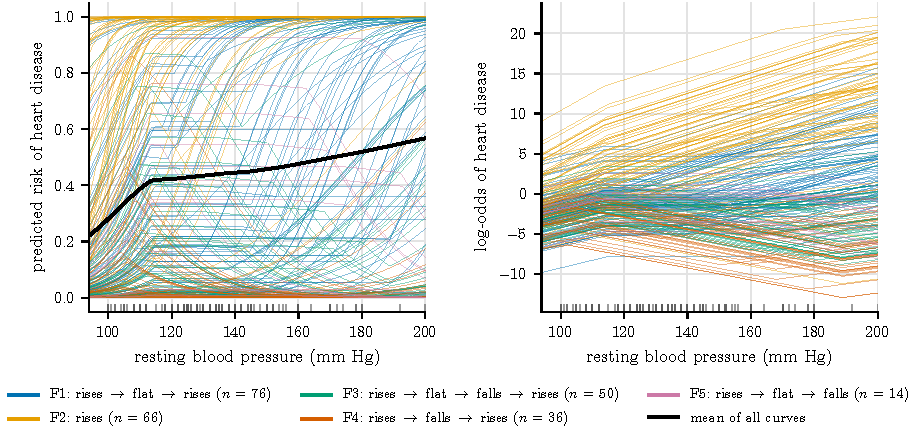
\includegraphics[width=\textwidth]{figures/exp2/exp2-s8-ice}
  \caption{Heart-100 seed 8: each of the 242 training patients' predicted risk as resting blood pressure varies with everything else about the patient held (individual conditional expectation curves), coloured by shape family (Table~\ref{tab:exp2-s8-families}). Ticks on the axis: the patients' own values; only 13 lie above 160~mm~Hg, so the late falls and rises rest on few patients. The curves are the model's, not a claim about blood pressure.}
  \label{fig:exp2-s8-ice}
\end{figure}

% Generated by experiments/exp2_thesis/make_assets.py -- do not edit by hand.
\begin{figure}[tbp]
  \centering
  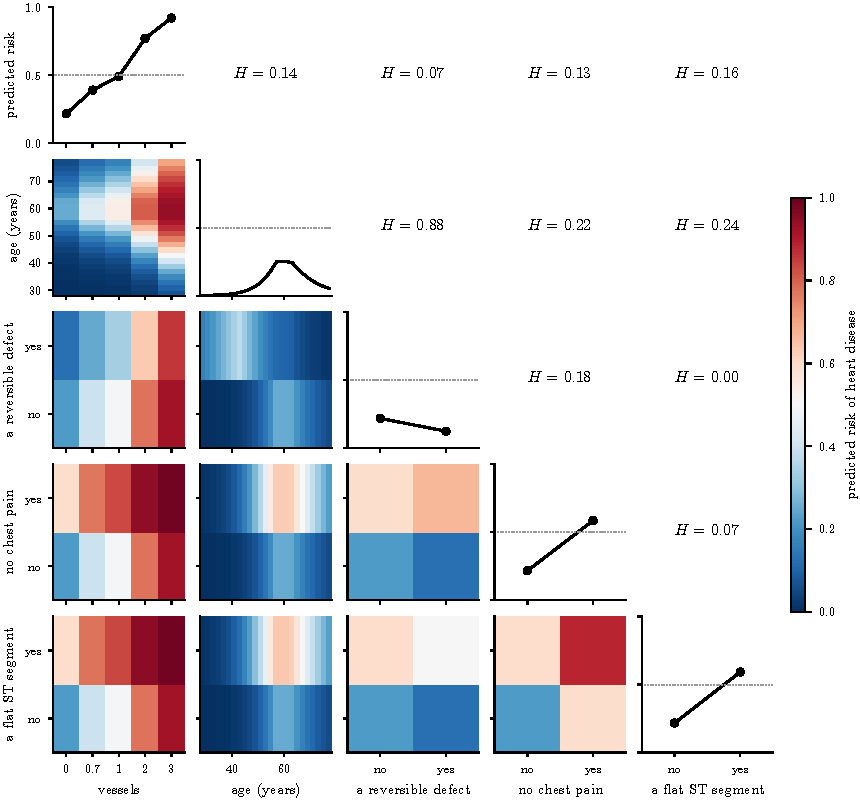
\includegraphics[width=0.95\textwidth]{figures/exp2/exp2-heart-pairs}
  \caption{Heart-100 seed 2, the whole model: a pairs plot over the five inputs it is most sensitive to. Diagonal: predicted risk as one input varies; below the diagonal: as two vary together (colour, centred on a risk of 0.5); other inputs held at their training median, which is a reference patient with a predicted risk of 0.22. Above the diagonal: the strength of each pair's interaction ($H$, the share of the pair's variation not explained by the two inputs separately, weighted by where the data lie). The strongest is age with a reversible defect.}
  \label{fig:exp2-heart-pairs}
\end{figure}

\clearpage
\section*{Churn}
% Generated by experiments/exp2_thesis/make_assets.py -- do not edit by hand.
\begin{table}[tbp]
  \centering
  \footnotesize
  \begin{tabularx}{\textwidth}{@{}>{\raggedright\arraybackslash}Xcccc@{}}
    \toprule
    Signal & \makecell{Relevance\\(CV)} & \makecell{Seeds\\using} & \makecell{Gain, median\\train / test} & \makecell{Seeds with test\\CI $>0$ ($<0$)} \\
    \midrule
    \multicolumn{5}{@{}l}{\textit{Core: used by every seed}} \\
    \quad International plan, offset & $+$0.040 & 10 & 0.064 / 0.075 & 10 \\
    \quad Service calls, slope & $+$0.027 & 10 & 0.025 / 0.034 & 10 \\
    \quad Service-call threshold & $+$0.022 & 10 & 0.010 / 0.009 & 3 \\
    \quad Heavy-day hinge & $+$0.017 & 10 & 0.014 / 0.018 & 7 \\
    \quad Day usage, slope & $+$0.015 & 10 & 0.010 / 0.007 & 3 \\
    \quad Evening usage, slope & $+$0.012 & 10 & 0.003 / 0.009 & 8 \\
    \quad Voice mail, offset & $+$0.010 & 10 & 0.005 / 0.006 & 2 \\
    \quad State offsets$^\dagger$ & $-$0.001 & 10 & 0.009 / $-$0.005 & 0 (1) \\
    \quad Night usage, slope & $-$0.003 & 10 & 0.001 / 0.004 & 5 \\
    \midrule
    \multicolumn{5}{@{}l}{\textit{Common: used by 4 to 9 seeds}} \\
    \quad Day $+$ evening bill & $+$0.024 & 9 & 0.008 / 0.007 & 3 \\
    \quad Service calls $\times$ light day use & $+$0.021 & 9 & 0.008 / 0.010 & 9 \\
    \quad International minutes, slope & $+$0.010 & 9 & 0.002 / 0.002 & 0 \\
    \quad Evening bend$^\dagger$ & $-$0.006 & 7 & $-$0.001 / 0.002 & 0 \\
    \quad Day calls, slope$^\dagger$ & $+$0.002 & 6 & 0.001 / $-$0.003 & 0 (3) \\
    \quad Account length, slope & $+$0.001 & 5 & 0.001 / $-$0.001 & 0 \\
    \quad Heavy day use without voice mail & $+$0.020 & 4 & 0.006 / 0.006 & 3 \\
    \quad International calls, slope & $+$0.001 & 4 & 0.001 / 0.001 & 0 \\
    \midrule
    \multicolumn{5}{@{}l}{\textit{Rare: used by 1 to 2 seeds}} \\
    \quad Service calls $\times$ voice mail$^\dagger$ & $-$0.000 & 2 & $-$0.000 / 0.001 & 0 \\
    \quad Evening usage $\times$ service calls$^\dagger$ & $-$0.003 & 2 & 0.001 / 0.000 & 0 \\
    \quad International-minutes bend & $+$0.008 & 1 & 0.000 / 0.000 & 0 \\
    \quad Day $\times$ night usage & $+$0.008 & 1 & 0.001 / $-$0.001 & 0 \\
    \midrule
    \multicolumn{5}{@{}l}{\textit{Absent from every network (relevant in the data)}} \\
    \quad International plan $\times$ international use & $+$0.047 & 0 & \multicolumn{2}{c}{data's own: test 0.015 [0.003, 0.026]} \\
    \quad International-calls bend & $+$0.003 & 0 & \multicolumn{2}{c}{data's own: test 0.004 [$-$0.003, 0.013]} \\
    \bottomrule
  \end{tabularx}
  \caption{Churn: the signals of the ten networks. A signal is a churn-relevant function of the inputs, defined on the data and independent of any model. \emph{Relevance}: the cross-validated log-loss gain when the signal is added to a ridge logistic fit on the training rows. A seed \emph{uses} a signal when its own component has a standard deviation of at least 0.10 logit. \emph{Gain}: AUC lost when that component is removed (median over the seeds using it). $^\dagger$Noise: the data do not support it or it never helps on test. The strongest interaction in the data, international plan $\times$ international use, is in no network.}
  \label{tab:exp2-churn-signals}
\end{table}

% Generated by experiments/exp2_thesis/make_assets.py -- do not edit by hand.
\begin{table}[tbp]
  \centering
  \footnotesize
  \begin{adjustbox}{max width=\textwidth}
  \setlength{\tabcolsep}{3pt}
  \begin{tabular}{@{}lcccccccccccc@{}}
    \toprule
    Seed & \rotatebox{70}{Calls slope} & \rotatebox{70}{Calls threshold} & \rotatebox{70}{Calls $\times$ light day} & \rotatebox{70}{Day slope} & \rotatebox{70}{Day hinge} & \rotatebox{70}{Day $+$ eve bill} & \rotatebox{70}{Day w/o voice mail} & \rotatebox{70}{Evening} & \rotatebox{70}{Intl plan} & \rotatebox{70}{Voice mail} & \rotatebox{70}{State} & \rotatebox{70}{Plan $\times$ intl use} \\
    \midrule
    s0 & 0.73 & \makecell{0.53\\{\scriptsize S4/3p}} & \makecell{0.33\\{\scriptsize S3/2p}} & 0.53 & \makecell{0.86\\{\scriptsize S4/3p}} & \makecell{0.40\\{\scriptsize S2/1p}} & \makecell{0.24\\{\scriptsize H/1p}} & 0.32 & 0.82 & 0.50 & 0.51 & -- \\
    s1 & 0.72 & \makecell{0.57\\{\scriptsize S2/1p}} & \makecell{0.33\\{\scriptsize H/1p}} & 0.66 & \makecell{0.99\\{\scriptsize S4/2p}} & \makecell{0.40\\{\scriptsize S2/1p}} & \makecell{0.38\\{\scriptsize H/1p}} & 0.45 & 0.85 & 0.45 & 0.51 & -- \\
    s2 & 0.85 & \makecell{0.60\\{\scriptsize S8/4p}} & \makecell{0.41\\{\scriptsize S6/3p}} & 0.56 & \makecell{0.80\\{\scriptsize S4/2p}} & \makecell{0.38\\{\scriptsize S4/2p}} & -- & 0.37 & 0.79 & 0.74 & 0.60 & -- \\
    s3 & 0.74 & \makecell{0.40\\{\scriptsize G/1p}} & \makecell{0.29\\{\scriptsize S3/2p}} & 0.68 & \makecell{0.74\\{\scriptsize S3/1p}} & \makecell{0.40\\{\scriptsize S2/1p}} & -- & 0.29 & 0.78 & 0.55 & 0.53 & -- \\
    s4 & 0.69 & \makecell{0.43\\{\scriptsize G/1p}} & \makecell{0.10\\{\scriptsize G/1p}} & 0.87 & \makecell{0.64\\{\scriptsize G/1p}} & \makecell{0.44\\{\scriptsize S2/1p}} & -- & 0.38 & 0.77 & 0.58 & 0.63 & -- \\
    s5 & 0.81 & \makecell{0.56\\{\scriptsize S4/1p}} & \makecell{\textbf{0.69}\\{\scriptsize S5/1p}} & 0.68 & \makecell{0.71\\{\scriptsize S4/2p}} & -- & -- & 0.48 & 0.78 & 0.60 & 0.47 & -- \\
    s6 & 0.88 & \makecell{0.50\\{\scriptsize S4/1p}} & \makecell{0.47\\{\scriptsize S5/2p}} & 0.55 & \makecell{0.86\\{\scriptsize S2/2p}} & \makecell{0.39\\{\scriptsize G/1p}} & \makecell{0.49\\{\scriptsize G/1p}} & 0.33 & 0.92 & 0.52 & 0.69 & -- \\
    s7 & 0.74 & \makecell{0.52\\{\scriptsize S2/2p}} & \makecell{0.25\\{\scriptsize S3/2p}} & 0.84 & \makecell{0.84\\{\scriptsize S5/3p}} & \makecell{0.50\\{\scriptsize S5/3p}} & \makecell{0.63\\{\scriptsize S5/3p}} & 0.25 & 0.88 & 0.41 & 0.55 & -- \\
    s8 & 0.68 & \makecell{0.53\\{\scriptsize S4/2p}} & \makecell{0.37\\{\scriptsize S4/2p}} & 0.51 & \makecell{0.64\\{\scriptsize S2/2p}} & \makecell{0.27\\{\scriptsize G/1p}} & -- & 0.32 & 0.70 & 0.57 & 0.59 & -- \\
    s9 & 0.61 & \makecell{0.48\\{\scriptsize H/1p}} & -- & 0.67 & \makecell{0.58\\{\scriptsize S5/2p}} & \makecell{0.30\\{\scriptsize S4/1p}} & -- & 0.29 & 0.76 & 0.47 & 0.54 & -- \\
    \bottomrule
  \end{tabular}
  \end{adjustbox}
  \caption{Churn: how each seed realises the main signals. Each cell is the standard deviation of the network's own component for that signal (logit, training rows). For a non-linear signal the second line gives its realisation: H, a single hinge on one input; G, a single gate (one unit that also reads another input); S$k$, split across $k$ units; /$n$p, spread over $n$ explanation parts. w: weak (0.03 to 0.10 logit); --: not used. Bold: the strongest calls $\times$ light-day realisation (s5). Every seed has the same core signals, assembled differently; no seed has the international plan $\times$ international use interaction.}
  \label{tab:exp2-churn-matrix}
\end{table}

% Generated by experiments/exp2_thesis/make_assets.py -- do not edit by hand.
\begin{figure}[tbp]
  \centering
  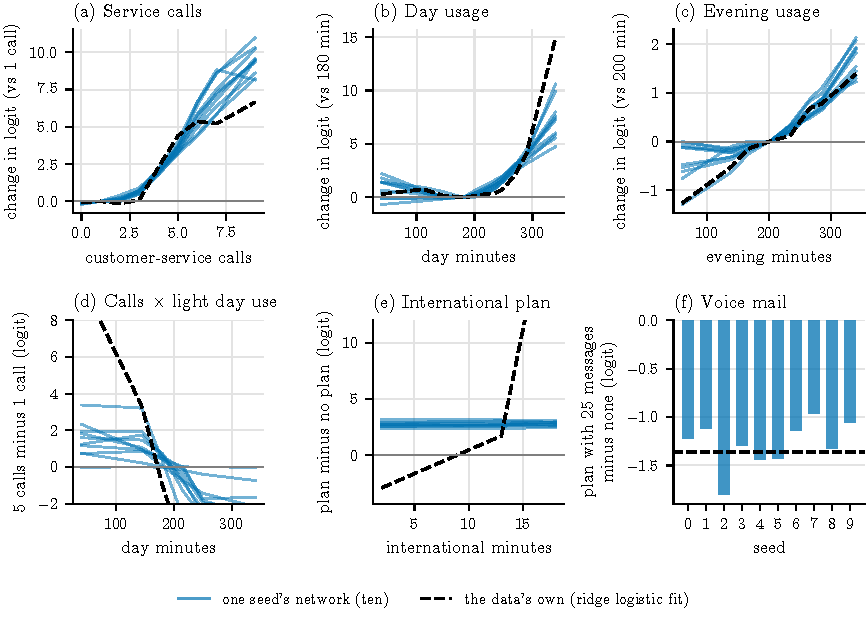
\includegraphics[width=\textwidth]{figures/exp2/exp2-churn-shapes}
  \caption{Churn: each signal's shape as realised in the ten networks (one line per seed), against the data's own shape (dashed). Each curve is the network's component for that signal, projected on the training rows, as a change in the churn score (logit); other inputs are at their training mean. (a)--(c) and (f) agree closely across seeds. (d) The seeds share one shape for calls $\times$ light day use, weaker than the data's. (e) Every network treats the international plan as a flat offset, while the data's effect rises steeply among plan holders with more than 13 international minutes (the interaction in Table~\ref{tab:exp2-churn-blindspot}); the data's curve is a ridge fit and extrapolates where customers are few.}
  \label{fig:exp2-churn-shapes}
\end{figure}

% Generated by experiments/exp2_thesis/make_assets.py -- do not edit by hand.
\begin{figure}[tbp]
  \centering
  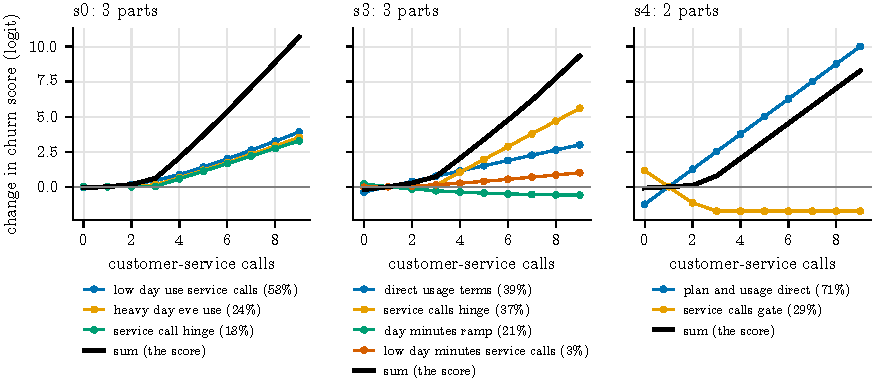
\includegraphics[width=\textwidth]{figures/exp2/exp2-churn-calls-parts}
  \caption{Churn: one signal, three realisations. The score's response to customer-service calls (mean over training customers, relative to 1 call) is split into the explanation parts that carry it; the parts sum exactly to the score's response (black). Seed 0 spreads the threshold over three parts, seed 3 builds it from a direct slope, a threshold hinge and a day-usage ramp, and in seed 4 a gate cancels the direct slope at low call counts (the two parts point in opposite directions; cancellation ratio 0.19). Legend: each part's share of the response's variance.}
  \label{fig:exp2-churn-calls-parts}
\end{figure}

% Generated by experiments/exp2_thesis/make_assets.py -- do not edit by hand.
\begin{figure}[tbp]
  \centering
  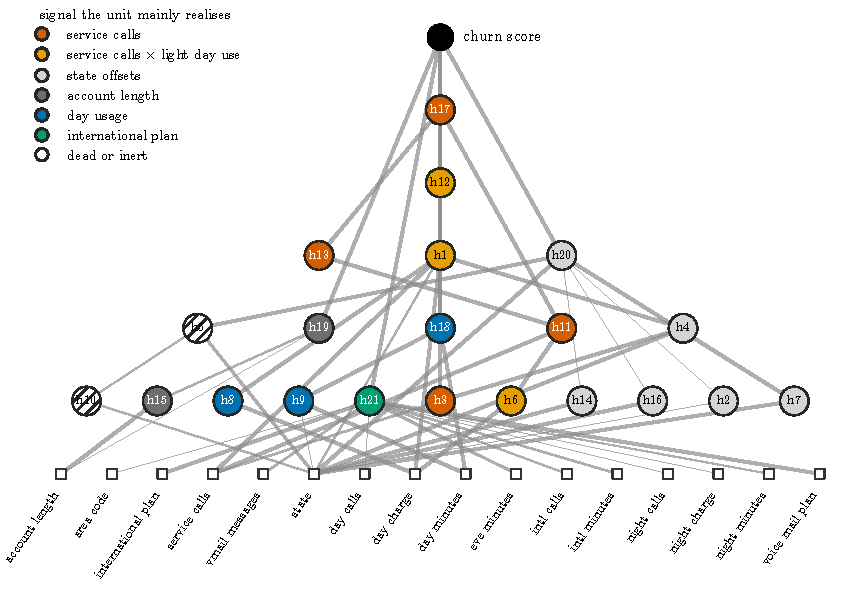
\includegraphics[width=\textwidth]{figures/exp2/exp2-churn-s5-network}
  \caption{Churn seed 5: every hidden node (21, labelled h1 to h21 as in the plain-language report) coloured by the signal it mainly realises; the 31 state indicators it reads are drawn as one input and line width follows the absolute weight. The service-call threshold and its interaction with light day use are built from 6 units (h1, h3, h6, h11, h12, h13); the identity nodes added by the explanation (h17, h18, h19, h20, h21) gather each part's output.}
  \label{fig:exp2-churn-s5-network}
\end{figure}

% Generated by experiments/exp2_thesis/make_assets.py -- do not edit by hand.
\begin{table}[tbp]
  \centering
  \small
  \begin{tabularx}{\textwidth}{@{}Xccc@{}}
    \toprule
    & \makecell{Share of\\disagreement} & \multicolumn{2}{c}{\makecell{Agreement after replacing it\\by the ten-seed average}} \\
    \cmidrule(l){3-4}
    Source of disagreement & & \makecell{Median logit\\correlation} & \makecell{Median top-141\\overlap} \\
    \midrule
    As trained & -- & 0.890 & 79\% \\
    \midrule
    State offsets & 22\% & 0.912 & 83\% \\
    Heavy-usage complex: day slope and hinge, day $+$ evening bill, day without voice mail, evening & 38\% & 0.935 & 83\% \\
    Service-call complex: slope and threshold, calls $\times$ light day use & 15\% & 0.906 & 84\% \\
    Night and international usage & 6\% & 0.897 & 82\% \\
    Other signals: voice mail, international plan, account and call counts, minor interactions & 8\% & -- & -- \\
    Residual: not in the signal list (three-way and state $\times$ usage gates) & 11\% & -- & -- \\
    \midrule
    Every signal except the state offsets & -- & 0.962 & 90\% \\
    Every signal (only the residual differs) & -- & 0.990 & 94\% \\
    State inputs held at their training average & -- & 0.909 & 80\% \\
    \bottomrule
  \end{tabularx}
  \caption{Churn: where the ten networks disagree, on the 1{,}000 test customers. Each pair's difference in logit is split into the signals' contributions; a signal's share is the covariance of its difference with the total difference over the variance of the total (mean over the 45 pairs; the shares sum to one). The right-hand columns replace that signal's realisation in every network by the ten-seed average and measure agreement again; the top-141 overlap compares each pair's 141 riskiest customers (the number who churned). Holding the state inputs at their average also raises the median test AUC from 0.886 to 0.894.}
  \label{tab:exp2-churn-disagreement}
\end{table}

% Generated by experiments/exp2_thesis/make_assets.py -- do not edit by hand.
\begin{table}[tbp]
  \centering
  \small
  \begin{tabular}{@{}lc@{}}
    \toprule
    \multicolumn{2}{@{}l}{\textit{Churn on the training rows}} \\
    International plan, at most 2 international calls & 69 of 69 (100\%) \\
    International plan, more than 13 international minutes & 66 of 66 (100\%) \\
    International plan, neither & 33 of 252 (13\%) \\
    No international plan & 405 of 3{,}620 (11\%) \\
    \midrule
    \multicolumn{2}{@{}l}{\textit{Test AUC}} \\
    Ridge logistic fit on the signal list, with this interaction & 0.922 \\
    The ten networks & 0.873--0.904 \\
    Their mean prediction & 0.899 \\
    \bottomrule
  \end{tabular}
  \caption{Churn: the signal no network has. Customers with an international plan churn almost surely when they make few international calls or many international minutes; every network treats the plan as a flat offset instead. This interaction is the most relevant signal in the data (cross-validated log-loss gain $+$0.047), and removing it from the ridge fit costs 0.015 test AUC [0.003, 0.026]. No network was trained with it, so its value to a network is untested.}
  \label{tab:exp2-churn-blindspot}
\end{table}

% Generated by experiments/exp2_thesis/make_assets.py -- do not edit by hand.
\begin{table}[tbp]
  \centering
  \small
  \begin{tabularx}{\textwidth}{@{}>{\raggedright\arraybackslash}Xccc@{}}
    \toprule
    & Churn & \makecell{Churn, state inputs\\at their average} & Heart-100 \\
    \midrule
    Test rows & 1{,}000 & 1{,}000 & 61 \\
    Logit correlation between seeds, median (min) & 0.890 (0.779) & 0.909 (0.792) & 0.921 (0.867) \\
    Rank correlation between seeds, median & 0.860 & 0.879 & 0.934 \\
    Overlap of the top-$k$ riskiest, median (min)$^\dagger$ & 79\% (69\%) & 80\% (71\%) & 91\% (84\%) \\
    Mean absolute difference in predicted risk, median & 0.051 & 0.049 & 0.087 \\
    Test AUC of one seed, median (range) & \makecell{0.886\\(0.873--0.904)} & \makecell{0.894\\(0.882--0.907)} & \makecell{0.892\\(0.863--0.926)} \\
    Test AUC of the ten seeds' mean prediction & 0.899 & 0.904 & 0.904 \\
    \bottomrule
  \end{tabularx}
  \caption{Prediction agreement between the ten seeds on the test rows (45 pairs per study). $^\dagger$The top $k$ is the number of positive test cases: $k=141$ for Churn and $k=32$ for Heart-100. Heart-100's seeds agree more closely with one another than Churn's do; on Churn, holding the state inputs at their training average removes part of the disagreement and slightly raises accuracy.}
  \label{tab:exp2-agreement}
\end{table}

\end{document}
